\documentclass[../../main]{subfiles}

\begin{document}

\section{Electrical System Design}

At the core of an AGV’s electrical system are power management, motor control, 
and communication networks, all of which must be carefully designed to meet 
performance and safety requirements. The power system typically consists of 
a rechargeable battery, often lithium-ion or lead-acid, along with a Battery 
Management System (BMS) to monitor voltage, current, and temperature for 
optimal energy efficiency and longevity. Motor controllers regulate the 
movement of the drive and steering motors, ensuring smooth acceleration, 
precise navigation, and effective braking. Additionally, AGVs rely on a 
network of embedded controllers, sensors, and communication modules to 
process data in real time, enabling obstacle detection, localization, and 
coordination a central control system.

\section{Power Supply and Distribution System}

At the heart of the AGV's electrical design lies the 
power supply and distribution system, which serves as the backbone 
for all onboard functionalities. This system is responsible for 
storing, managing, and delivering electrical energy to various 
components, including motors, sensors, control systems, and 
communication modules. Given that AGVs must operate continuously 
for extended periods, the selection of battery technology, capacity, 
and management strategies plays a critical role in determining 
performance, efficiency, and reliability. The AGV must be able to 
complete all assigned tasks without running out of power, making 
energy efficiency and power optimization essential in the design. 

To ensure safe and efficient energy usage, the AGV's battery system 
must integrate a Battery Management System (BMS). 
This system continuously monitors key parameters such as voltage, 
current, temperature, and state of charge, ensuring that the battery 
operates within safe limits while optimizing power delivery. 

Equally important is the power distribution architecture, which 
ensures reliable and efficient energy delivery to all AGV subsystems. 
This involves designing robust wiring harnesses, fuses, circuit 
breakers, and connectors capable of handling dynamic load 
requirements during various operational phases.

The following section explores the key components of the AGV's 
power supply and distribution system, their functions, and how 
they contribute to the overall efficiency and reliability of the vehicle.

\subsubsection{Power distribution architecture (System architecture)}

A well-structured power distribution network minimizes voltage drops and energy 
losses, directly contributing to longer operating times and reduced 
downtime for recharging. Furthermore, if the expected task duration 
exceeds the battery capacity, solutions such as hot-swappable 
batteries or rapid charging stations should be considered to maintain 
uninterrupted operations.

Figure \ref{Standard architecture for AGV} illustrates an efficient 
power distribution system\cite{system_architecture}for an AGV. The architecture 
includes key components such as the battery, 
power management system, motor controllers, sensors, 
microcontroller, and embedded computer. The power 
supply must ensure reliable and continuous energy 
delivery while optimizing efficiency and minimizing losses.
The power requirements of an AGV are primarily determined by 
the embedded-PC, microcontroller, sensors, and motors. 
The microcontroller is responsible for low-level control, 
including direct motor actuation and sensor data acquisition. 
Additionally, it provides a programming interface for the 
embedded-PC, which has higher computational capabilities 
and is used for high-level tasks, such as motion planning 
and coordination.

Since the battery supplies direct current (DC), different 
power conversion techniques are required to meet the voltage 
demands of various components. The high-voltage DC motors 
require DC-DC boosters to step up the supplied voltage to 
the necessary operating level. Meanwhile, low-voltage components 
such as sensors, the microcontroller, and embedded-PC rely on 
DC voltage regulators to ensure stable power delivery. 
This architecture enables precise control over motor speed 
through pulse width modulation (PWM), allowing for 
efficient and adaptive movement of the AGV.

\begin{figure}[!ht]
    \centering
    \resizebox{1\textwidth}{!}{%
    \begin{circuitikz}
    \tikzstyle{every node}=[font=\small]
    \draw  (3.25,11) rectangle (7,10);
    \draw  (3.25,9.25) rectangle (7,8.25);
    \draw  (3.25,7.5) rectangle (4.75,6.5);
    \draw  (5.5,7.5) rectangle (7,6.5);
    \draw  (1.25,9.25) rectangle (2,8.25);
    \draw [->, >=Stealth, dashed] (3.75,7.5) -- (3.75,8.25);
    \draw [->, >=Stealth, dashed] (4.25,8.25) -- (4.25,7.5);
    \draw [->, >=Stealth, dashed] (6,7.5) -- (6,8.25);
    \draw [->, >=Stealth, dashed] (6.5,8.25) -- (6.5,7.5);
    \draw [->, >=Stealth, dashed] (4.75,9.25) -- (4.75,10);
    \draw [->, >=Stealth, dashed] (5.5,10) -- (5.5,9.25);
    \draw  (0.5,11) rectangle (-0.5,6.5);
    \draw [short] (1.25,8.25) -- (2,9.25);
    \draw [short] (2.5,10.5) -- (2.5,7);
    \draw [->, >=Stealth] (2,8.75) -- (3.25,8.75);
    \draw [->, >=Stealth] (2.5,10.5) -- (3.25,10.5);
    \draw [->, >=Stealth] (2.5,7) -- (3.25,7);
    \draw [->, >=Stealth] (0.5,8.75) -- (1.25,8.75);
    \draw [short] (0,6.5) -- (0,5.5);
    \draw [->, >=Stealth] (6.25,5.5) -- (6.25,6.5);
    \draw  (2.75,6) rectangle (3.5,5);
    \draw [short] (3.5,5.5) -- (6.25,5.5);
    \draw [short] (2.75,5) -- (3.5,6);
    \draw [->, >=Stealth] (0,5.5) -- (2.75,5.5);
    \node [font=\small] at (1.5,9) {DC};
    \node [font=\small] at (1.75,8.5) {DC};
    \node [font=\small] at (3,5.75) {DC};
    \node [font=\small] at (3.25,5.25) {DC};
    \node [font=\normalsize, rotate around={90:(0,0)}] at (0,8.5) {Battery };
    \node [font=\normalsize] at (5.25,10.5) {Embedded-PC};
    \node [font=\normalsize] at (5.25,8.75) {Microcontroller};
    \node [font=\normalsize] at (4,7) {Sensors};
    \node [font=\normalsize] at (6.25,7) {Motors};
    \draw [->, >=Stealth] (8.75,10.5) -- (9.75,10.5);
    \draw [->, >=Stealth, dashed] (8.75,9.75) -- (9.75,9.75);
    \draw  (8.75,9.25) rectangle (9.5,8.25);
    \draw [short] (8.75,8.25) -- (9.5,9.25);
    \node [font=\small] at (9,9) {DC};
    \node [font=\small] at (9.25,8.5) {DC};
    \node [font=\normalsize] at (11.75,10.5) {Electric Power Flow};
    \node [font=\normalsize] at (11.5,9.75) {Information Flow};
    \node [font=\normalsize] at (13.25,8.75) {DC Converter (Booster or Regulator)};
    \end{circuitikz}
    }%
    \caption[AGV power distribution architecture.]{Typical architecture of an automated guided vehicle in terms of
    the electrical power distribution.}
    \label{Standard architecture for AGV}
    \end{figure}

\newpage
    \begin{figure}[!ht]
        \centering
        \rotatebox{90}{
        \resizebox{1.4\textwidth}{!}{%
        \begin{circuitikz}
        \tikzstyle{every node}=[font=\large]
        % \node (tikzmaker) [shift={(0, --1)}] at (4.5,21.5) {\includegraphics[width=0cm]{Raspberry}};
        \draw  (-33.75,7) rectangle  node {\large ESP32 S3-DevKit C1} (-28.75,5.25);
        \draw  (-27.5,7) rectangle  node {\large ESP32 S3-DevKit C1} (-22.5,5.25);
        \draw  (-39,13) rectangle  node {\large Husky Lens Camera} (-34.25,11.25);
        \draw  (-39,11) rectangle  node {\large QR Code reader} (-34.25,9.25);
        \draw  (-8.75,3.75) rectangle  node {\large Nema 23 Stepper Motor} (-3,1.75);
        \draw  (-53.5,3.75) rectangle  node {\large Nema 23 Stepper Motor} (-47.5,1.75);
        \draw  (-20,3.75) rectangle  node {\large Closed Loop Stepper Driver CL57T V4.1} (-10.75,1.75);
        \draw  (-45.5,3.75) rectangle  node {\large Closed Loop Stepper Driver CL57T V4.1} (-36.25,1.75);
        \draw  (-51.25,8.5) rectangle  node {\large Electric Linear Actuator } (-45,6.75);
        \draw  (-43.75,8.5) rectangle  node {\large BTS7960B Motor Driver Board} (-36.25,6.75);
        \draw  (-45.5,6.25) rectangle  node {\large 8 Channel Relay Card:} (-40.25,4.25);
        \draw  (-40.25,18) rectangle  node {\large 12V 70 AH AGM BATTERY} (-33.75,15.5);
        \draw  (-21.25,19.75) rectangle  node {\large WM-045 DC-DC 150W Voltage Step Up Module} (-10,17.5);
        \draw  (-50.5,-0.5) rectangle  node {\large 87dB 90X39mm Speaker:} (-41.75,-3);
        \draw  (-21.25,15.5) rectangle  node {\large 500W 30A DC-DC Constant Booster} (-13,13.25);
        \draw  (-20,9) rectangle  node {\large QTRX-HD-11RC} (-16.25,7.25);
        \draw  (-22,11) rectangle  node {\large LCD Screen} (-17,9.5);
        \draw  (-22,12.75) rectangle  node {\large RP LIDAR Sensor} (-17,11.25);
        \draw  (-27.5,0) rectangle  node {\large 9 Axis IMU } (-23.5,-1.75);
        \draw  (-20,6.75) rectangle  node {\large ToF Distance Sensor} (-14.25,4.25);
        \draw  (-32,18) rectangle (-24.25,15.5);
        \draw  (-31.75,12.25) rectangle  node {\large Raspberry-Pi 4 Model B} (-24.5,9.75);
        \node [font=\large] at (-27.75,16.75) {Battery Management System};
        \draw [->, >=Stealth] (-33.75,16.75) -- (-32,16.75);
        \draw [short] (-24.25,16.75) -- (-22.5,16.75);
        \draw [short] (-22.5,18.5) -- (-22.5,14.75);
        \draw [->, >=Stealth] (-22.5,18.5) -- (-21.25,18.5);
        \draw [->, >=Stealth] (-22.5,14.75) -- (-21.25,14.75);
        \draw [->, >=Stealth] (-29.5,15.5) -- (-29.5,12.25);
        \draw [->, >=Stealth, dashed] (-26.25,15.5) -- (-26.25,12.25);
        \draw [->, >=Stealth, dashed] (-30.75,9.75) -- (-30.75,7);
        \draw [->, >=Stealth, dashed] (-29.5,7) -- (-29.5,9.75);
        \draw [->, >=Stealth, dashed] (-27,7) -- (-27,9.75);
        \draw [->, >=Stealth, dashed] (-25.75,9.75) -- (-25.75,7);
        \draw [->, >=Stealth, dashed] (-34.25,11.75) -- (-31.75,11.75);
        \draw [->, >=Stealth, dashed] (-34.25,10.5) -- (-31.75,10.5);
        \draw [->, >=Stealth, dashed] (-22,10.5) -- (-24.5,10.5);
        \draw [->, >=Stealth, dashed] (-22,11.75) -- (-24.5,11.75);
        \draw [->, >=Stealth, dashed] (-43.75,7.5) -- (-45,7.5);
        \draw [dashed] (-32.5,7.75) -- (-32.5,7.25);
        \draw [dashed] (-32.5,5.25) -- (-32.5,2.5);
        \draw [->, >=Stealth, dashed] (-33.75,5.75) -- (-40.25,5.75);
        \draw [->, >=Stealth, dashed] (-32.5,7.75) -- (-36.25,7.75);
        \draw [->, >=Stealth, dashed] (-32.5,2.5) -- (-36.25,2.5);
        \draw [->, >=Stealth, dashed] (-33.25,3.25) -- (-33.25,5.25);
        \draw [dashed] (-36.25,3.25) -- (-33.25,3.25);
        \draw [dashed] (-23.75,2.5) -- (-23.75,5.25);
        \draw [dashed] (-23,3.25) -- (-20,3.25);
        \draw [->, >=Stealth, dashed] (-23,3.25) -- (-23,5.25);
        \draw [->, >=Stealth, dashed] (-23.75,2.5) -- (-20,2.5);
        \draw [->, >=Stealth, dashed] (-45.5,2.75) -- (-47.5,2.75);
        \draw [->, >=Stealth, dashed] (-10.75,2.75) -- (-8.75,2.75);
        \draw [->, >=Stealth] (-46.5,4.75) -- (-46.5,-0.5);
        \draw [short] (-46.5,4.75) -- (-45.5,4.75);
        \draw [short] (-45.5,5.5) -- (-50.25,5.5);
        \draw [short] (-45.5,6) -- (-47.5,6);
        \draw [->, >=Stealth] (-47.5,6) -- (-47.5,6.75);
        \draw [->, >=Stealth] (-50.25,5.5) -- (-50.25,3.75);
        \draw [short] (-40.25,4.5) -- (-24.75,4.5);
        \draw [short] (-24.75,4.5) -- (-24.75,0.75);
        \draw [short] (-24.75,0.75) -- (-7.75,0.75);
        \draw [->, >=Stealth] (-7.75,0.75) -- (-7.75,1.75);
        \draw [->, >=Stealth, dashed] (-25.5,0) -- (-25.5,5.25);
        \draw [short] (-48.25,20.75) -- (-15.5,20.75);
        \draw [short] (-13,14.75) -- (-6.25,14.75);
        \draw [->, >=Stealth] (-6.25,14.75) -- (-6.25,3.75);
        \draw [short] (-21.25,13.75) -- (-56.25,13.75);
        \draw [short] (-56.25,13.75) -- (-56.25,2.75);
        \draw [->, >=Stealth] (-56.25,2.75) -- (-53.5,2.75);
        \draw [short] (-15.5,20.75) -- (-15.5,19.75);
        \draw [->, >=Stealth] (-48.25,20.75) -- (-48.25,8.5);
        \node [font=\large] at (-32.5,12.25) {I2C};
        \node [font=\large] at (-32.5,11) {I2C};
        \node [font=\large] at (-23.75,12.25) {I2C};
        \node [font=\large] at (-31.5,9.25) {I2C};
        \node [font=\large] at (-25,9.25) {I2C};
        \draw [->, >=Stealth, dashed] (-20,6) -- (-22.5,6);
        \draw [->, >=Stealth, dashed] (-23.5,8) -- (-23.5,7);
        \draw [dashed] (-23.5,8) -- (-20,8);
        \draw  (-40.25,20.25) rectangle  node {\large TP-Link TL-WR840N} (-33.75,18.5);
        \draw [short] (-29.5,18) -- (-29.5,19.25);
        \draw [->, >=Stealth] (-29.5,19.25) -- (-33.75,19.25);
        \draw  (-33.75,1.25) rectangle  node {\large Load Cell Sensors} (-28.75,-0.5);
        \draw [->, >=Stealth, dashed] (-31.5,1.25) -- (-31.5,5.25);
        \node [font=\large] at (-30.75,4) {I2C};
        \node [font=\large] at (-26.25,4) {I2C};
        \draw  (-47,12) rectangle  node {\large Remote PC} (-41.25,10.25);
        \draw [dashed] (-44.25,14.5) -- (-30.5,14.5);
        \draw [->, >=Stealth, dashed] (-44.25,14.5) -- (-44.25,12);
        \draw [->, >=Stealth, dashed] (-30.5,14.5) -- (-30.5,12.25);
        \node [font=\large] at (-38,15) {WIFI};
        \node [font=\large] at (-21.5,6.5) {I2C};
        \node [font=\large] at (-21.75,8.5) {UART};
        \node [font=\large] at (-22.5,1.75) {UART};
        \node [font=\large] at (-36.75,5.25) {UART};
        \end{circuitikz}
        }%
        }
        % \caption{ Electrical power distribution architecture of the CIU_Fox, highlighting key components such as the battery, motor controllers, sensors, and embedded systems.} 
        \label{Actual system architecture}
        \caption{Actual system architecture}
        \end{figure}


The CIU\_Fox robot features a sophisticated electrical and control system integrating multiple 
embedded components, sensors, and power management units to ensure efficient operation. 
At the core of its control system are two ESP32 S3-DevKit C1 microcontrollers, responsible for 
handling various sensor inputs and executing real-time processing. These microcontrollers 
communicate with a Raspberry Pi 4 Model B, which serves as the main computational unit, 
facilitating high-level processing and decision-making. The Raspberry Pi is interconnected with 
several peripherals through I2C and UART communication protocols, ensuring seamless data 
transmission between components such as the Husky Lens camera, QR code reader, and RP 
LIDAR sensor, which contribute to the robot's vision and navigation capabilities. Additionally, 
an LCD screen displays real-time feedback (Sensors output,error message,...), while a 9-axis IMU enhances motion sensing for 
precise movement adjustments.

For actuation, the robot relies on Nema 23 stepper motors, which are powered and controlled 
by Closed Loop Stepper Driver CL57T V4.1 modules, ensuring precise rotational movements. 
These motors work in conjunction with an electric linear actuator (Lifting mechanism) controlled via a BTS7960B 
motor driver board. To manage additional mechanical operations and ensure safety, an 8-channel relay card is integrated into the system. 
This relay card not only coordinates multiple control signals for precise operation but also serves as a critical safety feature by isolating 
power components, such as motors and brakes, from the main circuit in case of an emergency. This dual functionality ensures both reliable control 
and robust fail-safe protection during operation. The CIU\_Fox robot is also equipped with load cell sensors, allowing it to measure 
forces applied to its lifting mechanism. 

Distance sensing and obstacle avoidance are managed by a Time-of-Flight (ToF) sensor and a LiDAR system, which together provide precise environmental 
awareness for navigation and object detection. Complementing these systems, the QTRX-HD-11RC modules work alongside the camera to deliver robust 
line-following capabilities, ensuring accurate path tracking and reliable navigation in structured environments.

A 12V 70AH AGM battery serves as the primary power source, 
delivering energy to various subsystems. A Battery Management 
System (BMS) regulates power flow, preventing overcharging 
and ensuring optimal energy usage. Voltage regulation is 
achieved using a combination of modules, including a WM-045 
DC-DC 150W step-up converter, a 500W 30A DC-DC constant 
booster, and LM2576 buck converters for 3.3V, 5V, and 9V 
outputs, ensuring stable and precise voltage levels for all 
components. To enhance system functionality, an 87dB speaker 
is integrated, providing auditory alerts or notifications as 
needed. Wireless connectivity is established through a 
TP-Link TL-WR840N router, enabling remote access and control 
via a connected PC, which facilitates real-time monitoring 
and decision-making.

\subsubsection{Battery Management System (BMS)}

The \textbf{BMS} is integrated to monitor and manage the battery's health, 
ensuring safe and reliable operation. It oversees critical parameters such as voltage, current, and temperature,
preventing issues like overcharging, over-discharging, and overheating. Having a BMS typically optimizes battery performance, 
extending battery life by up to 30\% and supporting over 3500 charge-discharge cycles at 90\% Depth of Discharge (DOD). 
It also ensures safe operations with features like overcurrent protection, overvoltage protection, and temperature monitoring. 
Additionally, the BMS in this system includes a charging system that complies with the competition specifications, 
which supports an \textbf{AGM Battery} with a nominal voltage of \textbf{12VDC} and a charging current of \textbf{10A}.


\subsection{Battery System}

Battery selection is a key factor in the efficiency and reliability of an AGV system. 
Among the available options, Absorbent Glass Mat (AGM) and Gel (GEL) batteries, 
both types of Sealed Lead-Acid (SLA) or Valve-Regulated Lead-Acid (VRLA) batteries, 
stand out for their maintenance-free, leak-proof design and low self-discharge rate. 
While both are deep-cycle batteries capable of discharging up to 80\% of their capacity, 
GEL batteries emphasize durability and stable power delivery, whereas AGM batteries 
support higher discharge rates and slightly faster charging. 
However, neither is well-suited for opportunity charging, as frequent partial recharges reduce their lifespan.

For AGVs operating in controlled, single-shift environments, 
GEL batteries provide a strong balance between safety, longevity, and consistent performance, 
making them an optimal choice. They typically last 8--16 hours per charge, depending on the AGV type, 
and require a full recharge when reaching 40--50\% depth of discharge (DOD). 
While their charging time is slower (e.g., a 100Ah battery takes about 3 hours at 0.3C), 
their deep-cycle capability ensures steady, long-term operation, minimizing the need for frequent replacements.

Considering the AGV’s operational demands and the competition's specified battery requirements, 
AGM batteries are selected for this application. The competition specifies the following parameters: 
\textit{Battery Type: AGM Battery, Battery Voltage (Nominal): 12VDC, Battery Charging Current: 10A}.

\begin{figure}[H]
    \centering
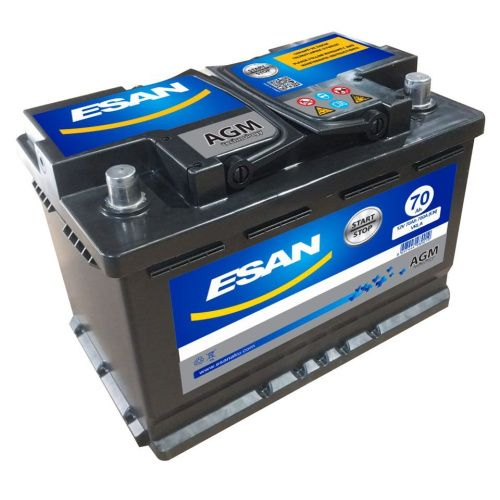
\includegraphics[width=0.45\textwidth]{fig/battery.jpg}
\caption{AGM battery}
\label{AGM battery} % Unique label for referencing
\end{figure}


\subsection{Voltage Regulation}

The AGV's electrical system contains various components operating 
at different voltage levels, making voltage regulation and 
distribution critical for stable operation. The majority of 
sensors operate at 3.3V to 5V, while components like the Raspberry Pi 
and ESP32 require 5V and others like the Wi-Fi router operates at 9V. 
To accommodate these diverse requirements, multiple voltage regulators 
are incorporated to step down the 12V battery supply to the appropriate 
levels, ensuring consistent performance across all subsystems. 


The \textbf{LM2596} in Figure~\ref{LM2596} voltage regulator will be used to step down the 12V battery 
supply to the required voltage levels for various components. Different 
versions of the LM2596 are available, including fixed output versions 
(9V, 5V, and 3.3V) as well as an adjustable version, allowing flexibility 
to meet the specific voltage requirements of each subsystem. For example, 
the 5V version will power the Raspberry Pi and ESP32, while the 3.3V version 
will support sensors operating at lower voltages. In cases where multiple 
components require the same voltage and draw significant current, multiple 
LM2596 regulators are placed in parallel to increase the current supply 
capacity(Table\ref{LM2596 Voltage Regulator Specifications}).

\begin{figure} 
    \centering
    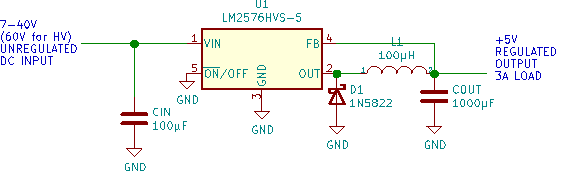
\includegraphics[width=0.7\textheight]{fig/lm2576.pdf}
    \caption{ Fixed Output Voltage Version Typical Application Diagram}
    \label{LM2596 Fixed Output Voltage} 
\end{figure}

\begin{figure} 
    \centering
    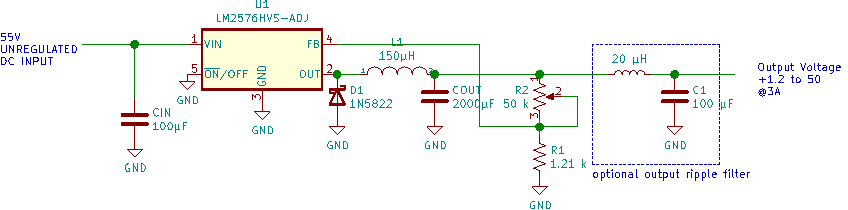
\includegraphics[width=0.7\textheight]{fig/lm2576_module_adj.pdf}
    \caption{1.2-V to 55-V Adjustable 3-A Power Supply With Low Output Ripple}
    \label{LM2596 Adjustable Output Voltage} 
\end{figure}

\begin{figure}[H]
    \centering
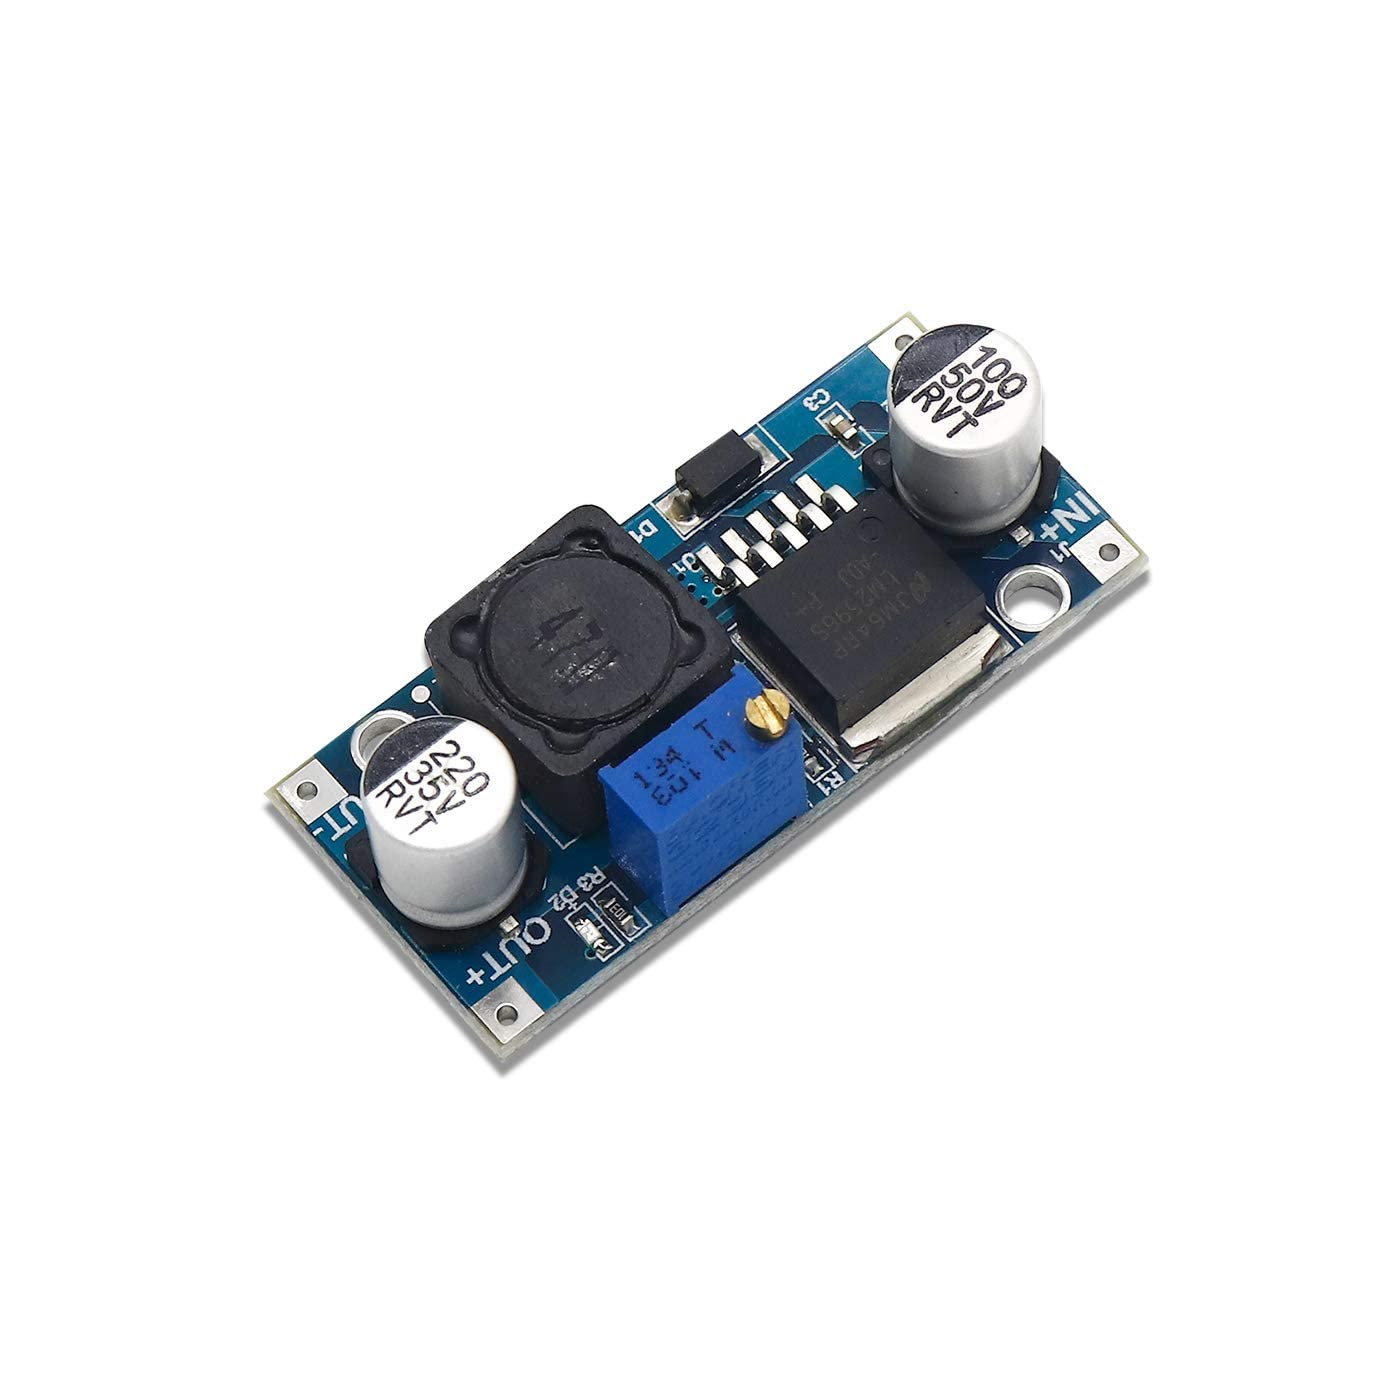
\includegraphics[width=0.5\textwidth]{fig/voltage_regulator.jpg}
\caption{LM2596 Voltage Regulator}
\label{LM2596} % Unique label for referencing
\end{figure}

\begin{table}[h!]
\centering
\begin{tabular}{|>{\bfseries}l|>{\ttfamily}l|}
\hline
Parameter & \multicolumn{1}{l|}{\textbf{Value}} \\ \hline
Input Voltage Range & Up to 40V \\ \hline
Output Current & Up to 3A \\ \hline
Switching Frequency & 150 kHz \\ \hline
Output Voltage Options & Fixed: 3.3V, 5V, 9V \\ 
 & Adjustable: 1.2V--37V \\ \hline
Efficiency & ~90\% \\ \hline
Protection Features & Thermal shutdown, current limiting \\ \hline
Package Type & TO-220, TO-263 \\ \hline
Operating Temperature & -40°C to +125°C \\ \hline
\end{tabular}
\caption{LM2596 Voltage Regulator Specifications}
\label{LM2596 Voltage Regulator Specifications} % Label for referencing
\end{table}

Furthermore, subsystems, such as the traction unit (composed of two stepper motors) 
and the lifting system (powered by linear actuators), require voltages 
higher than the battery's output. To address this, boost converters(\cref{Stepper motors booster} and \cref{Linear actuator booster}) are 
used to step up the voltage to the necessary levels. 

\begin{figure}[H]
    \centering
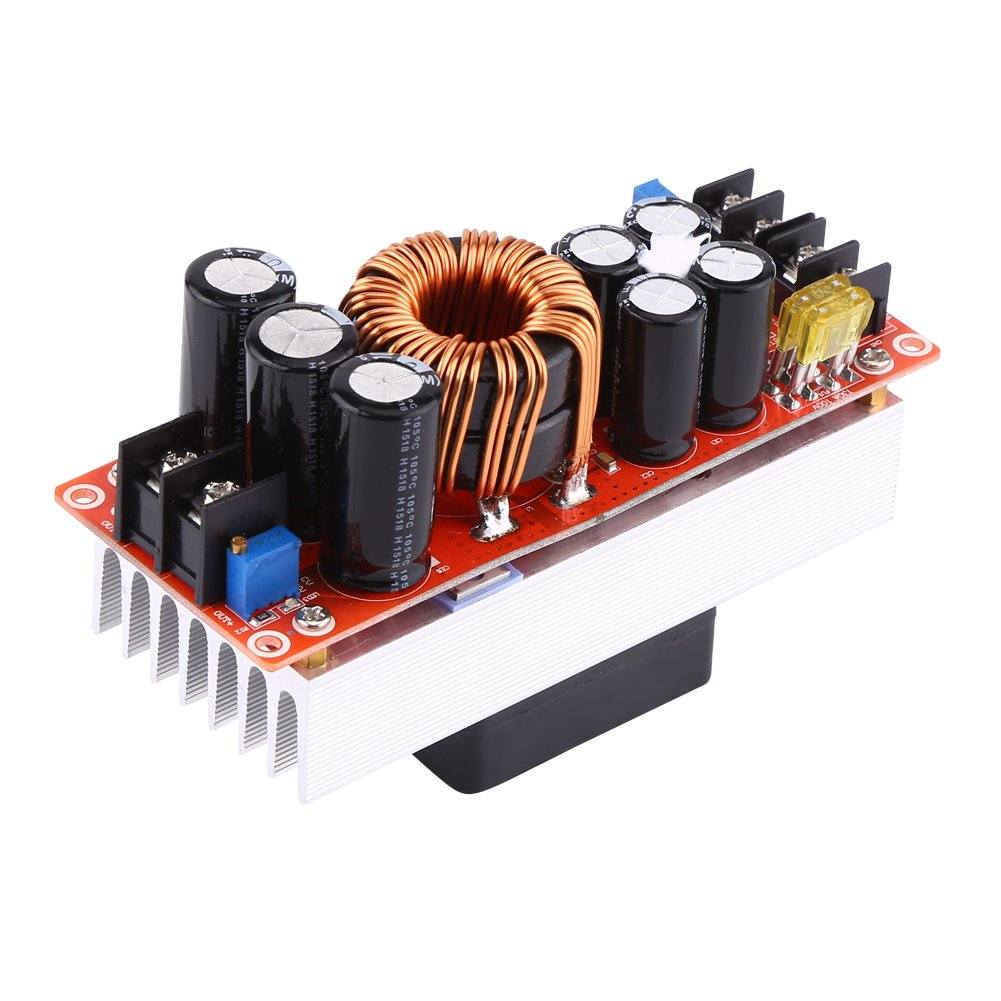
\includegraphics[width=0.5\textwidth]{fig/motor_booster.jpg}
\caption[1500W DC-DC Boost Converter (10-60V to 12-90V)]{1500W 30A DC-DC Constant Current Boost Converter Step-up Power Supply Module 10-60V to 12-90V }
\label{Stepper motors booster} % Unique label for referencing
\end{figure}


% \begin{table}[h!]
%     \centering
%     \begin{tabular}{|c|p{11cm}|} % Two columns with vertical lines
%         \hline
%         \textbf{Features:} & 
%         \parbox{11cm}{\centering
%         \vspace{5pt}
%             Flexible DC input voltage range from \texttt{10V} to \texttt{60V}; \\
%             Adjustable output voltage from \texttt{12V} to \texttt{90V} for versatile applications; \\
%             Maximum output current of \texttt{20A} for reliable power supply; \\
%             Built with high-power \texttt{100V/210A} low resistance MOS for efficiency; \\
%             Reverse input protection with MOS for added safety; \\
%             Low voltage protection to prevent damage from over-discharge; \\
%             Thickened heat sink and intelligent cooling fan for optimal heat dissipation.
%             \vspace{5pt}} \\ \hline
        
%         \textbf{Specifications:} & 
%         \parbox{10cm}{\centering \vspace{5pt}
%             Power: \texttt{1500W}; \\
%             Current: \texttt{30A}; \\
%             Input Voltage Range: \texttt{10V - 60V}; \\
%             Output Voltage Range: \texttt{12V - 90V}; \\
%             Maximum Output Current: \texttt{20A}. \vspace{5pt}
%         } \\ \hline
        
%         \textbf{Package Includes:} & 
%         \parbox{10cm}{\centering \vspace{5pt}
%             \texttt{1 × Boost Converter Step-up Power Supply Module}.
%             \vspace{5pt}} \\ \hline
%     \end{tabular}
%     \caption{DC-DC Constant Current Boost Converter Specifications and Features}
%     \label{tab:boost-converter-specs} % Label for referencing
% \end{table}
    
\begin{table}[h!]
    \centering
    \begin{tabular}{|>{\bfseries}l|p{10cm}|} % Two columns with vertical lines
    \hline
    Features: & 
    Flexible DC input voltage range from \texttt{10V} to \texttt{60V}; 
    Adjustable output voltage from \texttt{12V} to \texttt{90V} for versatile applications; 
    Maximum output current of \texttt{20A} for reliable power supply; 
    Built with high-power \texttt{100V/210A} low resistance MOS for efficiency; 
    Reverse input protection with MOS for added safety; 
    Low voltage protection to prevent damage from over-discharge; 
    Thickened heat sink and intelligent cooling fan for optimal heat dissipation. \\ \hline
    Specifications: & 
    Power: \texttt{1500W}; 
    Current: \texttt{30A}; 
    Input Voltage Range: \texttt{10V - 60V}; 
    Output Voltage Range: \texttt{12V - 90V}; 
    Maximum Output Current: \texttt{20A}. \\ \hline
    Package Includes: & 
    \texttt{ 1 × Boost Converter Step-up Power Supply Module}. \\ \hline
    \end{tabular}
    \caption{DC-DC Constant Current Boost Converter Specifications and Features}
    \label{Stepper motor booster specifications} % Label for referencing
\end{table}

\newpage
\begin{figure}[H]
    \centering
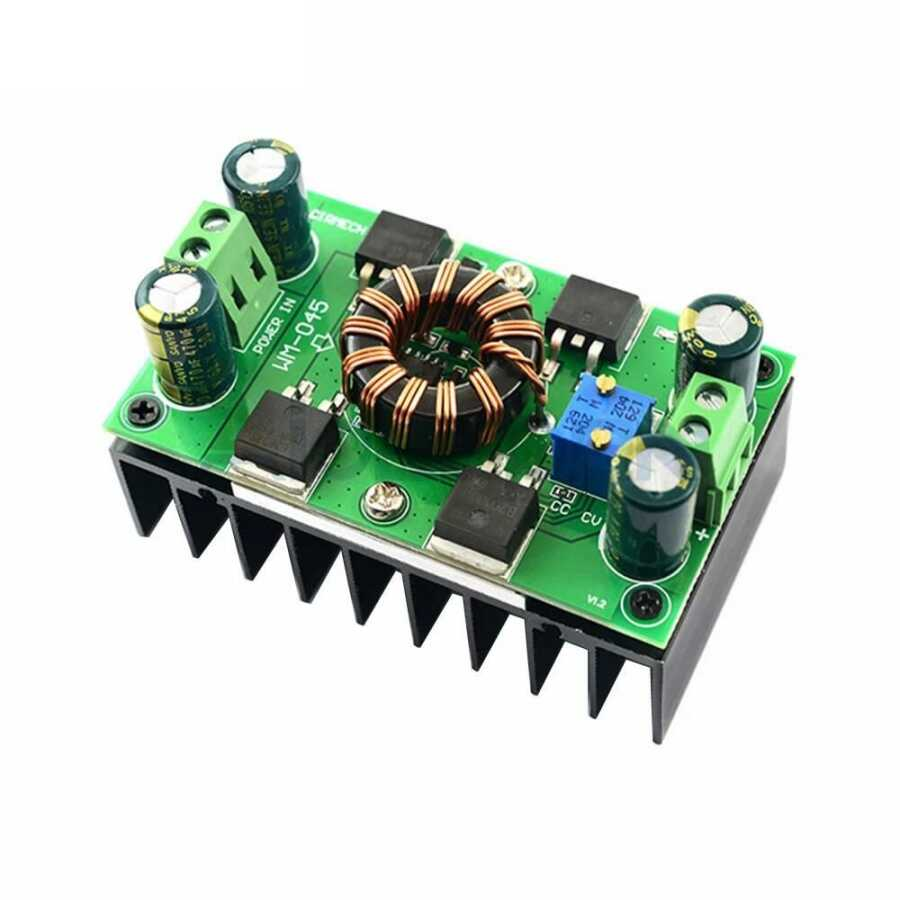
\includegraphics[width=0.55\textwidth]{fig/actuator_booster.jpg}
\caption{WM-045 DC-DC 150W Voltage Step Up and Step Down Regulator Module }
\label{Linear actuator booster} % Unique label for referencing
\end{figure}

% \begin{table}[ht]
%     \centering
%     \begin{tabular}{|c|p{10cm}|} % Two columns with vertical lines
%     \hline
%     \textbf{Features:} & \parbox{11cm}{\centering \vspace{5pt}
%     Input Voltage: \texttt{5Vdc ~ 30Vdc}; \\
%     Buck-Boost (automatic boost/lower); \\
%     Output Voltage: \texttt{1.25Vdc -- 30Vdc} (Adjustable);\\
%     Output Current: \texttt{10A (MAX)}.\vspace{5pt}} \\ \hline
%     \textbf{Specifications:} & \parbox{11cm}{\centering \vspace{5pt}
%     Output Power: \texttt{150W}; \\
%     Conversion Efficiency: \texttt{90\% Max}; \\
%     Ripple and Noise: \texttt{200mVp-p}; \\
%     No-Load Current: \texttt{6mA typical}.\vspace{5pt}} \\ \hline
%     \textbf{Performance Metrics:} & \parbox{11cm}{\centering \vspace{5pt}
%     Voltage Regulation: \texttt{± 0.5\%}; \\
%     Load Regulation: \texttt{± 0.5\%}; \\
%     Dynamic Response Rate: \texttt{300uS}.\vspace{5pt}} \\ \hline
%     \end{tabular}
%     \caption{Buck-Boost Converter Specifications}
%     \label{Linear actuator booster specifications} % Label for referencing
%     \end{table}

\begin{table}[htbp]
    \centering
    \begin{tabular}{|>{\bfseries}l|p{10cm}|} % Two columns with vertical lines
    \hline
    Features: & 
    Input Voltage: \texttt{5Vdc ~ 30Vdc}; 
    Buck-Boost (automatic boost/lower); 
    Output Voltage: \texttt{1.25Vdc ~ 30Vdc} (Adjustable); 
    Output Current: \texttt{10A (MAX)}. \\ \hline
    Specifications: & 
    Output Power: \texttt{150W}; 
    Conversion Efficiency: \texttt{90\% Max}; 
    Ripple and Noise: \texttt{200mVp-p}; 
    No-Load Current: \texttt{6mA typical}. \\ \hline
    Performance Metrics: & 
    Voltage Regulation: \texttt{± 0.5\%}; 
    Load Regulation: \texttt{± 0.5\%}; 
    Dynamic Response Rate: \texttt{300uS}. \\ \hline
    \end{tabular}
    \caption{Buck-Boost Converter Specifications}
    \label{Linear actuator booster specifications} % Label for referencing
    \end{table}

The power distribution circuits are designed to efficiently deliver power to all 
subsystems, including motors, sensors, controllers, and communication 
modules, while minimizing power losses and ensuring reliable operation. 
Protection circuits and fuses are also integrated to safeguard sensitive 
components from voltage spikes, short circuits, and other electrical faults, 
enhancing the overall safety and durability of the AGV.

\section{Motor Control System}

The performance and reliability of automated guided vehicles (AGVs) are deeply rooted in the precision and efficiency of
their motor control systems\cite{cservenak2018further}. At the heart of these systems lies the electrical design, which governs the interaction 
between power supply, control devices, and the physical dynamics of the motors. Direct current (DC) motors\cite{OrientalMotorAGV}, Stepper motors\cite{LinEngineering_AGV} and Servo motors\cite{AMC_AGV_Benefits}, widely 
used in AGVs due to their high torque, excellent speed regulation, and robust performance, require sophisticated electrical 
architectures to ensure optimal operation. 

From an electrical perspective, motor control involves not only the precise regulation of voltage and current but 
also the implementation of efficient drivers and motor controllers, which are critical for achieving smooth acceleration, 
stable speed control, and efficient energy utilization. Furthermore, the motor control system must address challenges 
such as minimizing power losses, managing heat dissipation, and ensuring reliable operation under varying load conditions. 

A motor control system comprises two fundamental components: the motors themselves and the motor drivers or controllers. 
The motor alone cannot achieve optimal operation without the integration of a sophisticated motor driver or controller. 
The motor driver acts as the intermediary between the power supply and the motor, regulating voltage and current to ensure 
smooth and efficient operation. It interprets control signals and translates them into precise commands.

\subsection{Motors and actuators}

The choice of motor depends on several factors, including torque requirements, speed, wheel size, load capacity, operating voltage, and environmental conditions. Below, we discuss the key considerations for motor selection in AGV applications.

\paragraph{Torque and Speed Requirements}
The motor must generate sufficient torque to move the AGV and its payload efficiently, overcoming rolling resistance and any potential obstacles. Simultaneously, it should achieve the desired speed without compromising torque. For instance, AGVs operating in environments with frequent stops and starts may require motors with high torque at low speeds, while those used in long-distance transportation may prioritize higher speed capabilities.

\paragraph{Wheel Size and Load Capacity}
The size and weight of the AGV wheels directly influence motor selection. Larger wheels and heavier payloads demand motors with higher torque and power ratings. Additionally, the motor must be capable of handling the AGV's maximum load capacity without overheating or losing efficiency.

\paragraph{Operating Voltage}
The motor's operating voltage must align with the AGV's power supply system. Common voltage options include 12V, 24V, and 48V. It is essential to choose a voltage that is both compatible with the AGV's design and readily available for the intended application.

\paragraph{Motor Types}
The two most common motor types for AGVs are DC motors and brushless DC (BLDC) motors. DC motors are cost-effective and straightforward, making them suitable for simpler applications. On the other hand, BLDC motors offer superior efficiency, longer lifespan, and smoother operation, making them ideal for more demanding AGV tasks. The choice between these motor types depends on the specific requirements of the AGV, such as precision, durability, and control complexity.

\paragraph{Control System Compatibility}
The selected motor must integrate seamlessly with the AGV's control system. This includes compatibility with communication protocols and interfaces, such as PWM (Pulse Width Modulation) for speed control or CAN bus for advanced communication. Ensuring compatibility is crucial for achieving precise control and coordination with other AGV subsystems.

\paragraph{Encoders and Feedback Mechanisms}
For AGVs requiring high precision and accurate path correction, motors equipped with encoders or feedback mechanisms are highly recommended. Encoders provide real-time data on the motor's position and speed, enabling closed-loop control and improved navigation accuracy. This feature is particularly important for AGVs operating in dynamic or complex environments.

\paragraph{Environmental Considerations}
The operating environment plays a significant role in motor selection. AGVs operating in harsh conditions, such as dusty or moist environments, require motors with appropriate protection ratings (e.g., IP65 or higher). Additionally, motors should be selected based on their ability to withstand temperature variations and mechanical stress.

\paragraph{Energy Efficiency}
Energy efficiency is a critical factor, especially for AGVs that operate for extended periods or rely on battery power. Motors with high efficiency reduce power consumption, extend battery life, and lower operational costs. BLDC motors, for example, are known for their energy-efficient performance compared to traditional DC motors.

\paragraph{Cost and Availability}
While selecting a motor, it is essential to balance performance requirements with budget constraints. Consider not only the initial cost of the motor but also its availability, maintenance requirements, and long-term reliability. Consulting with manufacturers and industry experts can help identify cost-effective solutions without compromising performance.

\subsubsection{Traction unit motors and linear actuator}


    
\paragraph{P Series Nema 23 Closed Loop Stepper Motor with Electromagnetic
    Brake (2Nm):}
    
    The traction system of the automated guided vehicle (AGV)  
    is driven by two NEMA 23 P-Series stepper motors shown Figure~\ref{Nema 23 stepper motor},  
    each delivering a holding torque of 2.0 Nm to ensure  
    reliable and precise motion. These motors are selected  
    for their high torque-to-size ratio, making them well-suited  
    for the dynamic demands of AGV operations.  
    
    Both motors are equipped with incremental encoders, which provide real-time feedback  
    on motor speed and position. This closed-loop system  
    enhances the AGV's ability to maintain smooth and synchronized  
    motion, ensuring stability and precision during navigation.  
    
    Additionally, each motor is integrated with an electromagnetic  
    brake, enabling rapid deceleration and enhancing safety  
    by halting motion instantly when required. 

\begin{figure}[H]
\centering
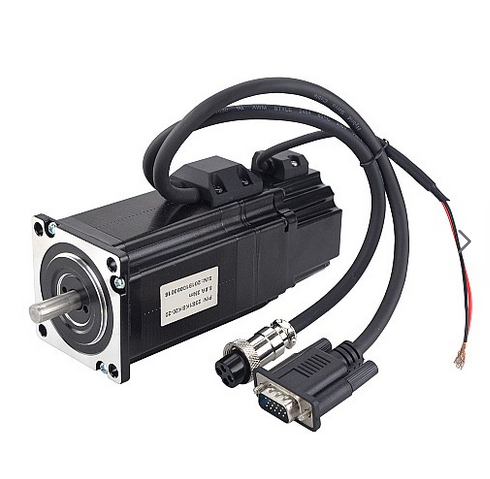
\includegraphics[width=0.4\textwidth]{fig/nema_motor.png}
\caption{Nema 23 stepper motor 2 Nm torque }
\label{Nema 23 stepper motor} % Unique label for referencing
\end{figure}

\begin{table}[h!]
    \centering
    \begin{tabular}{|>{\bfseries}l|>{\ttfamily}p{10cm}|} % Two columns with vertical lines
    \hline
    \multicolumn{2}{|c|}{\textbf{Electrical Specification}} \\ \hline
    Manufacturer Part Number & 23E1KBK20-20 \\ \hline
    Number of Phases & 2 \\ \hline
    Step Angle & 1.8deg \\ \hline
    Holding Torque & 2Nm (283.28oz.in) \\ \hline
    Rated Current/Phase & 5.0A \\ \hline
    Phase Resistance & 0.4ohms \\ \hline
    Inductance & 1.8mH ± 20\% (1KHz) \\ \hline
    Insulation Class & B 130°C [266°F] \\ \hline
    \multicolumn{2}{|c|}{\textbf{Physical Specification}} \\ \hline
    Frame Size & 57 x 57mm \\ \hline
    Body Length & 76.5mm \\ \hline
    Shaft Diameter & 8mm \\ \hline
    Shaft Length & 21mm \\ \hline
    D-Cut Shaft Length & 15mm \\ \hline
    Lead Length & 270mm \\ \hline
    Weight & 1.06kg \\ \hline
    \multicolumn{2}{|c|}{\textbf{Encoder Specification}} \\ \hline
    Output Circuit Type & Differential type \\ \hline
    Encoder Type & Incremental \\ \hline
    Output Signal Channels & 2 channels \\ \hline
    Supply Voltage Min & 5V \\ \hline
    Supply Voltage Max & 5V \\ \hline
    Output High Voltage & <4V \\ \hline
    Output Low Voltage & <1V \\ \hline
    \multicolumn{2}{|c|}{\textbf{Brake Connections}} \\ \hline
    Red--24V+ & Red--24V- \\ \hline
    Brake Torque & 2.0Nm \\ \hline
    \end{tabular}
    \caption{Stepper Motor Specifications (Model: 23E1KBK20-20)}
    \label{Nema 23 motor specifications} % Label for referencing
\end{table}

\newpage

paragraph{DC 12V Electric Linear Actuator (Maximum Force 6000N):}

The lifting mechanism of the automated guided vehicle (AGV)  
utilizes a high-performance linear actuator to achieve  
precise vertical motion. The actuator includes an overload  
protection feature, preventing excessive force application  
and minimizing mechanical wear.

\begin{figure}[h!]
    \centering
    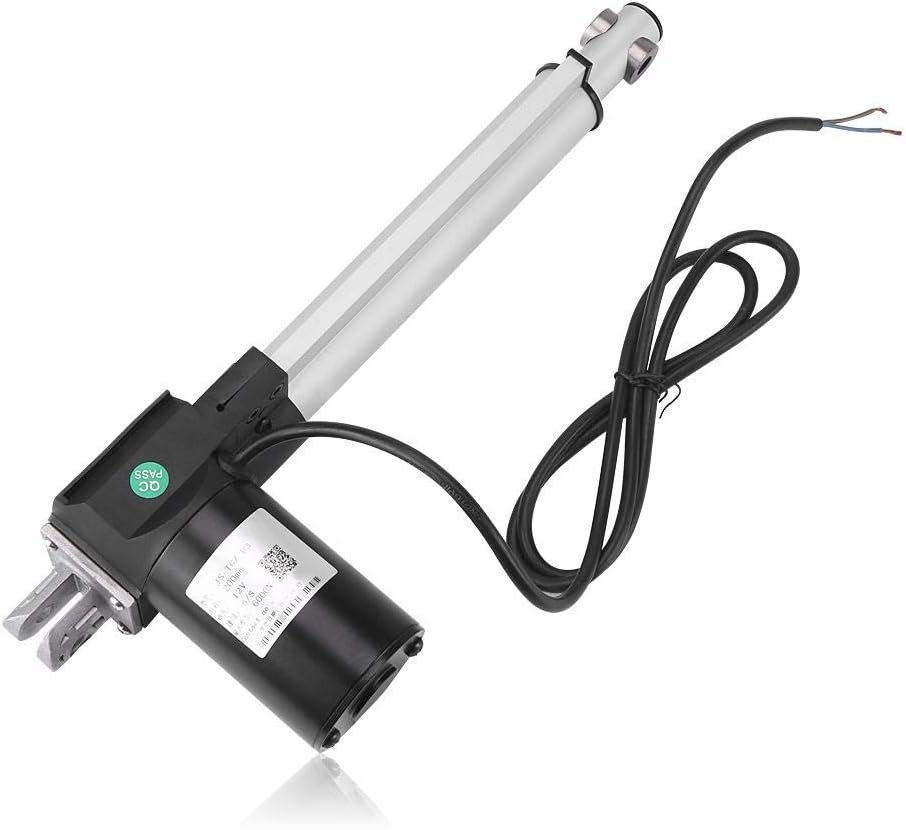
\includegraphics[width=0.45\textwidth]{fig/linear_actuator.jpg}
    \caption{Linear actuator with a maximum stoke of 6000N }
    \label{Linear actuator} % Unique label for referencing
\end{figure}

\begin{table}[h!]
    \centering
    \begin{tabular}{|>{\bfseries}l|>{\ttfamily}l|} % Two columns with vertical lines
    \hline
    Model & \texttt{JS-TGZ-U3} \\ \hline
    Material & \texttt{Metal} \\ \hline
    Voltage & \texttt{DC 12V} \\ \hline
    Maximum Push/Pull Force & \texttt{Approx. 6000N/6000N} \\ \hline
    Stroke & \texttt{450mm} \\ \hline
    No-Load Speed & \texttt{Maximum 5mm/s} \\ \hline
    Rated Load Rate & \texttt{5mm/s (600kg)} \\ \hline
    Environment Temperature & \texttt{-26°C to +65°C} \\ \hline
    Standard Protection Level & \texttt{IP54} \\ \hline
    Built-in Stroke Switch & \texttt{Yes} \\ \hline
    Color & \texttt{Silver} \\ \hline
    \end{tabular}
    \caption{Specifications of the linear actuator model JS-TGZ-U3}
    \label{Linear Actuator Specifications} % Label for referencing
    
\end{table}




\subsubsection{Motor Drivers and Controllers}


\paragraph{Closed Loop Stepper Driver V4.1 CL57T:}

The \textbf{Closed Loop Stepper Driver V4.1 CL57T} has been selected 
to complement the \textbf{Nema 23 Closed Loop Stepper Motor}, 
ensuring precise and reliable control over the AGV's propulsion and mechanical functions. 

From an electrical perspective, the CL57T driver leverages 
advanced closed-loop technology to guarantee accurate motor positioning, 
even in dynamic environments or when encountering external resistance. 
Fully compatible with software tools like \textbf{CLseries} and \textbf{Motion Studio}, 
the driver enables fine-tuning of critical motor parameters, optimizing performance 
for specific operational requirements. 

Additionally, its extensive diagnostic and monitoring ports provide 
real-time tracking of key electrical and operational metrics, 
such as \textbf{temperature}, \textbf{current}, \textbf{torque}, \textbf{RPM}, 
and overall motor state during operation. These capabilities not only enhance operational 
visibility but also streamline troubleshooting and diagnostics, minimizing downtime and ensuring swift resolution of issues. 




% \begin{table}[ht]
%     \centering
%     \begin{tabular}{|>{\bfseries}l|>{\ttfamily}p{8cm}|} % Two columns with vertical lines
%     \hline
%     \multicolumn{2}{|c|}{\textbf{Key Features}} \\ \hline
%     \multicolumn{2}{|p{10cm}|}{\texttt{RS232 debugging interface}} \\ 
%     \multicolumn{2}{|p{10cm}|}{\texttt{Do not need a high torque margin}} \\ 
%     \multicolumn{2}{|p{10cm}|}{\texttt{Broader operating speed range}} \\ 
%     \multicolumn{2}{|p{10cm}|}{\texttt{Reduced motor heating and more efficient}} \\ 
%     \multicolumn{2}{|p{10cm}|}{\texttt{Smooth motion and super-low motor noise}} \\ 
%     \multicolumn{2}{|p{12cm}|}{\texttt{5V/24V logic voltage selector, default setting 24V}} \\ 
%     \multicolumn{2}{|p{12cm}|}{\texttt{Closed-loop, eliminates loss of synchronization}} \\ 
%     \multicolumn{2}{|p{15cm}|}{\texttt{Protections for over-voltage,over-current,and position following error}} \\ 
%     \multicolumn{2}{|p{15cm}|}{\texttt{By default, supports an encoder with a resolution of 1000PPR; customizable between 0-5000PPR}} \\ 
%     \hline
    
%     \multicolumn{2}{|c|}{\textbf{Electrical Specifications}} \\ \hline
%     Output Peak Current & \texttt{0~8A} \\ \hline
%     Input Voltage & \texttt{+24~48VDC (Typical 36VDC)} \\ \hline
%     Logic Signal Current & \texttt{7~16mA (Typical 10mA)} \\ \hline
%     Pulse Input Frequency & \texttt{0~200kHz} \\ \hline
%     Isolation Resistance & \texttt{500Mohm} \\ \hline
    
%     \multicolumn{2}{|c|}{\textbf{Operating Environment and Other Specifications (Tj = 25°C/77°F)}} \\ \hline
%     Cooling & Natural Cooling or Forced Cooling \\ \hline
%     Environment & Avoid dust, oil mist, and corrosive gases \\ \hline
%     Ambient Temperature & \texttt{0°C - 65°C} \\ \hline
%     Humidity & \texttt{40\%RH - 90\%RH} \\ \hline
%     Operating Temperature & \texttt{0°C - 50°C} \\ \hline
%     Vibration & \texttt{10-50Hz / 0.15mm} \\ \hline
%     Storage Temperature & \texttt{-20°C - 65°C} \\ \hline
%     Weight & \texttt{Approx. 280g (9.9oz)} \\ \hline
%     \end{tabular}
%     \caption{Specifications of the Closed-Loop Stepper Driver}
%     \label{Stepper motor driver specifications} % Label for referencing
    
% \end{table}
    
\begin{table}[htbp]
    \centering
    \begin{tabular}{|>{\bfseries}l|>{\ttfamily}p{10cm}|} % Two columns with vertical lines
    \hline
    \multicolumn{2}{|c|}{\textbf{Key Features}} \\ \hline
     & RS232 debugging interface \\ 
     & Do not need a high torque margin \\ 
     & Broader operating speed range \\ 
     & Reduced motor heating and more efficient \\ 
     & Smooth motion and super-low motor noise \\ 
     & 5V/24V logic voltage selector, default setting 24V \\ 
     & Closed-loop, eliminates loss of synchronization \\ 
     & Protections for over-voltage, over-current, and position following error \\ 
     & By default, supports an encoder with a resolution of 1000PPR; customizable between 0-5000PPR \\ \hline
    
    \multicolumn{2}{|c|}{\textbf{Electrical Specifications}} \\ \hline
    Output Peak Current & \texttt{0~8A} \\ \hline
    Input Voltage & \texttt{+24~48VDC (Typical 36VDC)} \\ \hline
    Logic Signal Current & \texttt{7~16mA (Typical 10mA)} \\ \hline
    Pulse Input Frequency & \texttt{0~200kHz} \\ \hline
    Isolation Resistance & \texttt{500Mohm} \\ \hline
    
    \multicolumn{2}{|c|}{\textbf{Operating Environment and Other Specifications (Tj = 25°C/77°F)}} \\ \hline
    Cooling & Natural Cooling or Forced Cooling \\ \hline
    Environment & Avoid dust, oil mist, and corrosive gases \\ \hline
    Ambient Temperature & \texttt{0°C - 65°C} \\ \hline
    Humidity & \texttt{40\%RH - 90\%RH} \\ \hline
    Operating Temperature & \texttt{0°C - 50°C} \\ \hline
    Vibration & \texttt{10-50Hz / 0.15mm} \\ \hline
    Storage Temperature & \texttt{-20°C - 65°C} \\ \hline
    Weight & \texttt{Approx. 280g (9.9oz)} \\ \hline
    \end{tabular}
    \caption{Specifications of the Closed-Loop Stepper Driver}
    \label{Stepper motor driver specifications} % Label for referencing
    
\end{table}

\begin{figure}[H]
    \centering
    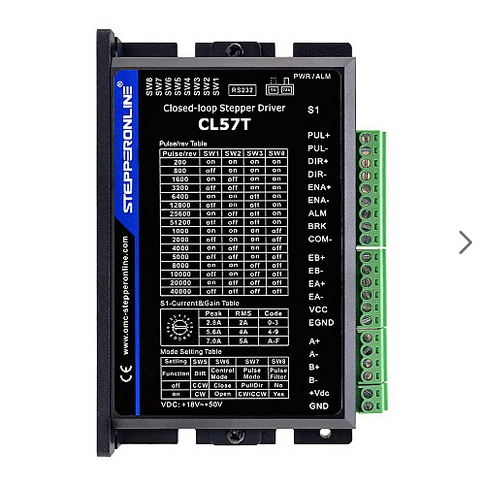
\includegraphics[width=0.45\textwidth]{fig/stepper_driver.png}
    \caption{ Closed Loop Stepper Driver CL57T V4.1 }
    \label{Stepper motor driver } % Unique label for referencing
\end{figure}

\paragraph{BTS7960B 40 Amp Motor Driver Board}

The BTS7960B 40A Motor Driver Board is selected for its capability to control 
high-power motors, making it ideal for the AGV’s linear actuator. 
Supporting currents up to 40A, it ensures reliable performance in demanding applications. 

\begin{figure}[H]
    \centering
    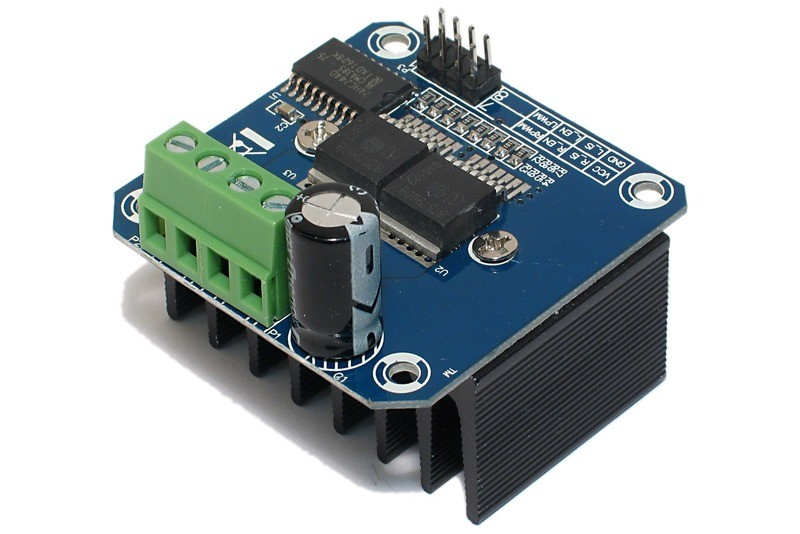
\includegraphics[width=0.45\textwidth]{fig/40_amp_driver.jpg}
    \caption{ DC-MOTOR DRIVER MODULE 24V 43A (2x BTS7960B) }
    \label{Linear actuator driver } % Unique label for referencing
\end{figure}


% \begin{table}[ht]
%     \centering
%     \begin{tabular}{|>{\bfseries}l|>{\ttfamily}p{10cm}|} % Two columns with vertical lines
%     \hline
%     \multicolumn{2}{|c|}{\textbf{Features}} \\ \hline
%     \multicolumn{2}{|p{15cm}|}{\texttt{Double BTS7960 large current (43A) H-bridge driver}} \\ 
%     \multicolumn{2}{|p{15cm}|}{\texttt{5V isolation with MCU, effectively protecting the MCU}} \\ 
%     \multicolumn{2}{|p{15cm}|}{\texttt{5V power indicator on board}} \\ 
%     \multicolumn{2}{|p{15cm}|}{\texttt{Voltage indication of motor driver output end}} \\ 
%     \multicolumn{2}{|p{15cm}|}{\texttt{Can solder heat sink for improved thermal management}} \\ 
%     \multicolumn{2}{|p{15cm}|}{\texttt{Requires only four lines from MCU to driver module (GND, 5V, PWM1, PWM2)}} \\ 
%     \multicolumn{2}{|p{15cm}|}{\texttt{Isolation chip 5V power supply (can share with MCU 5V)}} \\ 
%     \multicolumn{2}{|p{15cm}|}{\texttt{Supports motor forward and reverse control; two PWM input frequencies up to 25kHz}} \\ 
%     \multicolumn{2}{|p{15cm}|}{\texttt{Two heat flow passing through an error signal output}} \\ 
%     \multicolumn{2}{|p{15cm}|}{\texttt{On-board 5V supply can be used or shared with MCU 5V}} \\ \hline
%     \multicolumn{2}{|c|}{\textbf{Specifications}} \\ \hline
%     Model & \texttt{IBT-2} \\ \hline
%     Input Voltage & \texttt{6V - 27V} \\ \hline
%     Maximum Current & \texttt{43A} \\ \hline
%     Input Level & \texttt{3.3V - 5V} \\ \hline
%     Control Method & \texttt{PWM or level} \\ \hline
%     Duty Cycle & \texttt{0\% - 100\%} \\ \hline
%     Size & \texttt{4 x 5 x 1.2 cm / 1.6 x 2.0 x 0.5 inch} \\ \hline
%     \end{tabular}
%     \caption{Features and Specifications of the IBT-2 Motor Driver Module}
%     \label{Linear actuator specifications} % Label for referencing
    
% \end{table}

\begin{table}[htbp]
    \centering
    \begin{tabular}{|>{\bfseries}l|>{\ttfamily}p{10cm}|} % Two columns with vertical lines
    \hline
    \multicolumn{2}{|c|}{\textbf{Features}} \\ \hline
     & Double BTS7960 large current (43A) H-bridge driver \\ 
     & 5V isolation with MCU, effectively protecting the MCU \\ 
     & 5V power indicator on board \\ 
     & Voltage indication of motor driver output end \\ 
     & Can solder heat sink for improved thermal management \\ 
     & Requires only four lines from MCU to driver module (GND, 5V, PWM1, PWM2) \\ 
     & Isolation chip 5V power supply (can share with MCU 5V) \\ 
     & Supports motor forward and reverse control; two PWM input frequencies up to 25kHz \\ 
     & Two heat flow passing through an error signal output \\ 
     & On-board 5V supply can be used or shared with MCU 5V \\ \hline

    \multicolumn{2}{|c|}{\textbf{Specifications}} \\ \hline
    Model & \texttt{IBT-2} \\ \hline
    Input Voltage & \texttt{6V - 27V} \\ \hline
    Maximum Current & \texttt{43A} \\ \hline
    Input Level & \texttt{3.3V - 5V} \\ \hline
    Control Method & \texttt{PWM or level} \\ \hline
    Duty Cycle & \texttt{0\% - 100\%} \\ \hline
    Size & \texttt{4 x 5 x 1.2 cm / 1.6 x 2.0 x 0.5 inch} \\ \hline
    \end{tabular}
    \caption{Features and Specifications of the IBT-2 Motor Driver Module}
    \label{Linear actuator specifications} % Label for referencing
    
\end{table}
    
\newpage

\subsubsection{Motor Feedback and Braking Systems}
For precise control and safety, the AGV's motors are equipped with encoders and brakes. 
The two primary motors feature optical incremental encoders and power-off brakes, 
ensuring accurate feedback and reliable stopping mechanisms.

\paragraph{Encoder Specifications}
The motors utilize optical incremental encoders with the following specifications:


\begin{table}[htbp]
    \centering
    \begin{tabular}{|>{\bfseries}l|>{\ttfamily}p{10cm}|} % Two columns with vertical lines
    \hline
    \multicolumn{2}{|c|}{\textbf{Encoder Specifications}} \\ \hline
    Encoder Type & Optical Incremental \\ \hline
    Resolution & 1000 PPR (Pulses Per Revolution) \\ \hline
    Output Circuit Type & Differential \\ \hline
    Output Signal Channels & 2 \\ \hline
    \end{tabular}
    \caption{Encoder Specifications}
    \label{encoder_specifications} % Label for referencing
\end{table}

These encoders provide high-resolution feedback on motor position and speed, 
enabling precise control and navigation for the AGV.

\paragraph{Brake Specifications}
The motors are equipped with power-off brakes, which engage automatically in the event of a power failure, 
ensuring the AGV remains stationary. The brake specifications are as follows:

\begin{table}[htbp]
    \centering
    \begin{tabular}{|>{\bfseries}l|>{\ttfamily}p{10cm}|} % Two columns with vertical lines
    \hline
    \multicolumn{2}{|c|}{\textbf{Brake Specifications}} \\ \hline
    Brake Type & Power Off Brake \\ \hline
    Holding Torque & 200 Ncm \\ \hline
    Brake Rated Voltage & 24V \\ \hline
    Brake Current & 0.16A \\ \hline
    Brake Power & 4W \\ \hline
    Response Time & 50ms \\ \hline
    \end{tabular}
    \caption{Electromagnetic Brake Specifications}
    \label{brake_specifications} % Label for referencing
\end{table}

The brakes shown in Figure~\ref{ Electromagnetic Brake} provide a holding torque of 200 Ncm, ensuring the AGV remains stable even under load. 
he fast response time of 50ms guarantees quick engagement, enhancing safety during operation.

\begin{figure}[H]
    \centering
    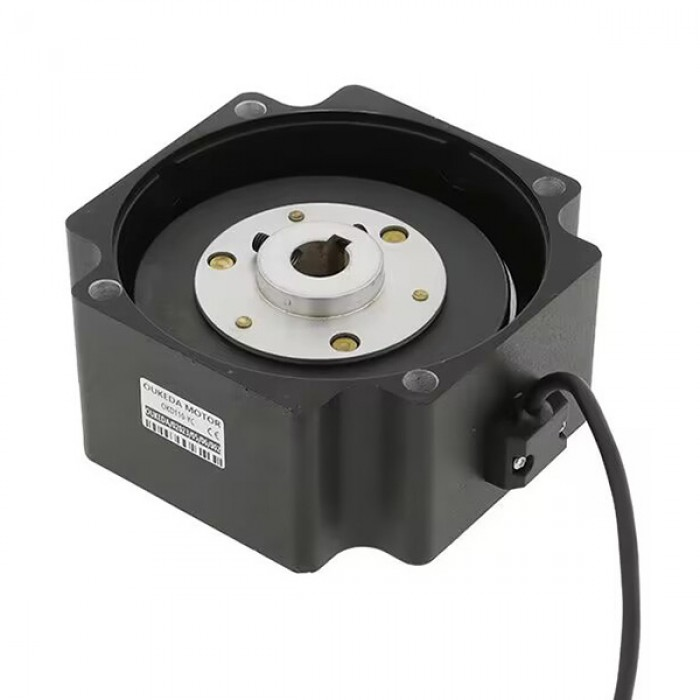
\includegraphics[width=0.5\textwidth]{fig/brakes.jpg}
    \caption{ Electromagnetic Brake for Nema 23 }
    \label{ Electromagnetic Brake} % Unique label for referencing
\end{figure}

The encoder feedback is integrated into the AGV's control system, enabling real-time monitoring and adjustment of motor performance. The brakes are designed to work seamlessly with the power supply, ensuring immediate activation during emergencies or power loss.

\section{Sensors}
Various sensors, such as LiDAR, cameras, and infrared sensors, are utilized for
navigation, obstacle detection, and localization.

The AGV is equipped with a variety of sensors to ensure accurate 
navigation, obstacle detection, weight measurement, and environmental 
perception. These sensors work together to enhance the robot's 
autonomy, safety, and efficiency. The following sensors are integrated 
into the system:

\subsection{VL53L0X (Time-of-Flight Distance Sensor)}

The VL53L0X time-of-flight (ToF) distance sensors  play an important role in enhancing 
the AGV's perception of its immediate surrounding in an operational perspective. 
hese sensors are strategically integrated into the AGV design by deploying eight 
ToF sensors—two at each corner of the robot insuring a comprehensive coverage. 
The ToF sensors are especially important in scenarios where traditional sensing methods, 
such as LiDAR, may be limited or rendered ineffective. For instance, when the AGV carries 
a lifted platform that obstructs the LiDAR's field of view, the ToF sensors take over to provide reliable distance measurements within a range of 0.5m to 12m . 
\begin{figure}[H]
    \centering
    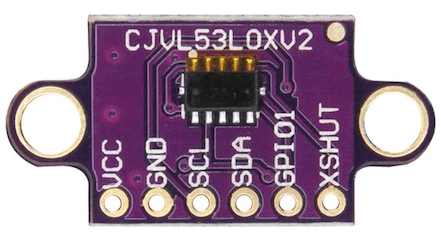
\includegraphics[width=0.45\textwidth]{fig/tof_sensor.png}
    \caption{ VL53L0X time-of-flight (ToF) distance sensor }
    \label{LVL53L0X ToF sensor } % Unique label for referencing
\end{figure}


\subsection{Weight Sensor - Load Sensor 50Kg}

This sensor provides accurate and continuous monitoring of the load on the AGV.

\begin{figure}[H]
    \centering
    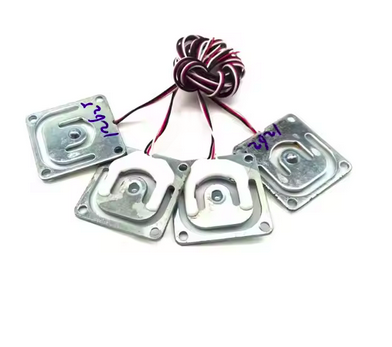
\includegraphics[width=0.45\textwidth]{fig/4_cells.png}
    \caption{ Load cell }
    \label{Load cell} % Unique label for referencing
\end{figure}

\begin{figure}[h!]
    \centering
    \begin{circuitikz}[scale=1.2, transform shape,american voltages]
  
        % Wheatstone Bridge
        \draw (0,0) to [R=$R_1$] (45:3); % Resistor R1
        \draw (0,0) to [R, l_=$R_2$] (-45:3); % Resistor R3
        \draw (45:3) to[R=$R_3$] ++(-45:3) coordinate(alpha); % Resistor R2
        \draw (alpha) to[R=$R_4$] (-45:3); % Resistor R4
  
        \draw (45:3) --++(0,0.5)  to [short, o-*] ++(-3,0)node[left]{$V_+$}; % Positive terminal
        \draw (-45:3)--++(0,-0.5)  to [short, o-*] ++(-3,0)node[left]{$V_-$}; % Positive terminal
  
        % \draw (0,0) to[open, v^=$V_{\text{out}}$, *-*] (alpha);
        \draw (0,0) to[rmeter, t=$V$] (alpha);
  
  
    \end{circuitikz}
    \caption{Load Cell Circuit with Wheatstone Bridge and Amplifier}
    \label{fig:load-cell}
  \end{figure}
  The idea behind the load cell is to use the Wheatstone bridge (\cref{fig:load-cell}). In a Wheatstone bridge, $R_1 = R_2 = R_3 = R_4$, and the output voltage is zero when no force is applied. When weight is applied, it bends the material, which changes the resistivity of the material. This change disrupts the equality of the resistances, causing a difference in voltage across $V$. By experimenting and calibrating with different weights and tracking the changes in voltage, we can measure the weight.

  It is also worth noting that the signal produced depends on the material properties. If the bending factor is linear, the output will be proportional to the applied weight. However, if the bending becomes exponential (which would be a limitation of the material), the relationship between the applied weight and the output signal may no longer be accurate. Additionally, the placement of the load affects the measurement. The voltage difference across $V$ is used to measure the output of the bridge.
  
  In theory, we could use the microcontroller's analog input to read the voltage differences. However, the changes are too small to provide an accurate reading. For this reason, the \textbf{HX711} amplifier is used to amplify the signal and convert it into a digital signal.

The HX711 in \cref{HX711 Load cell amplifier} is specifically designed to enhance the weak 
output signals from the load cellin \cref{Load cell}, ensuring accurate and reliable weight measurements.

\begin{figure}[H]
    \centering
    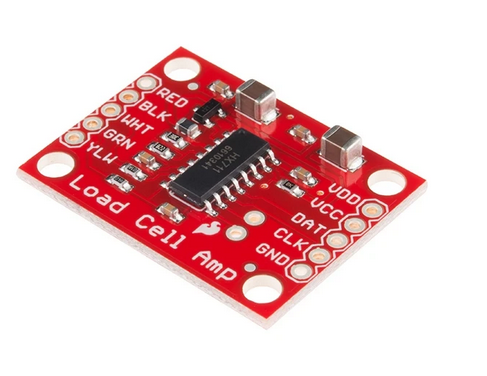
\includegraphics[width=0.45\textwidth]{fig/load_cell_amplifier.png}
    \caption{ HX711 Load cell amplifier }
    \label{HX711 Load cell amplifier} % Unique label for referencing
\end{figure}


\subsection{RPLIDAR - 360}

The RPLIDAR sensor provides comprehensive environmental mapping, making it indispensable for AGV navigation 
from an electrical control perspective. With its ability to deliver high-accuracy, real-time 360-degree
scanning, the RPLIDAR enables the AGV to perceive its surroundings with exceptional precision.

\begin{figure}[H]
    \centering
    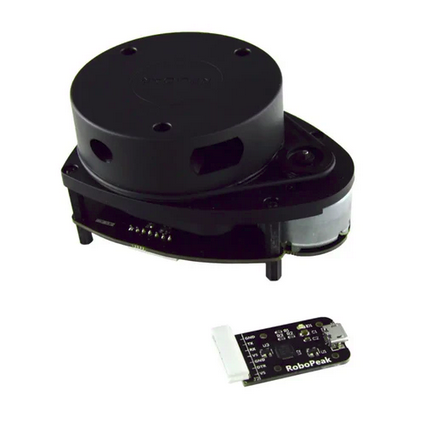
\includegraphics[width=0.45\textwidth]{fig/lidar.png}
    \caption{ RPLIDAR - 360}
    \label{ RPLIDAR - 360 } % Unique label for referencing
\end{figure}


\subsection{Camera HUSKYLENS}

The \textbf{HUSKYLENS} vision sensor enhances the AGV’s performance 
used for \textbf{object detection and line following}. 
It provides accurate real-time visual feedback, allowing dynamic adjustments to 
motor speed, direction, and trajectory. 

\begin{figure}[H]
    \centering
    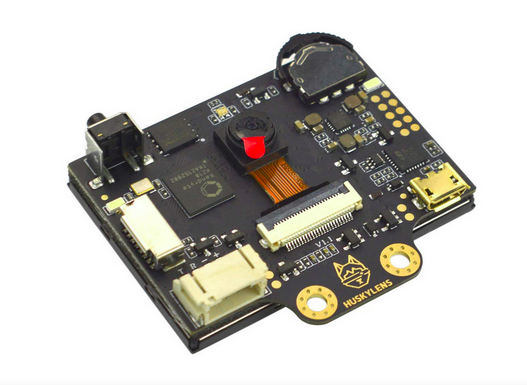
\includegraphics[width=0.5\textwidth]{fig/huskylens.png}
    \caption{ Huskylens camera}
    \label{ Huskylens camera} % Unique label for referencing
\end{figure}


\subsection{IMU Sensor}

The Inertial Measurement Unit (IMU)  is used for achieving precise positioning and movement control in automated guided vehicles (AGVs)
The MPU9255 integrates a 3-axis gyroscope, 3-axis accelerometer, and 3-axis magnetometer, providing comprehensive data on angular velocity, 
linear acceleration, and magnetic field orientation. The MPU9255 communicates with the AGV’s control system via I2C or SPI interfaces, 
ensuring low-latency data transmission while minimizing power consumption—a key consideration for energy-efficient operation.

\begin{figure}[H]
    \centering
    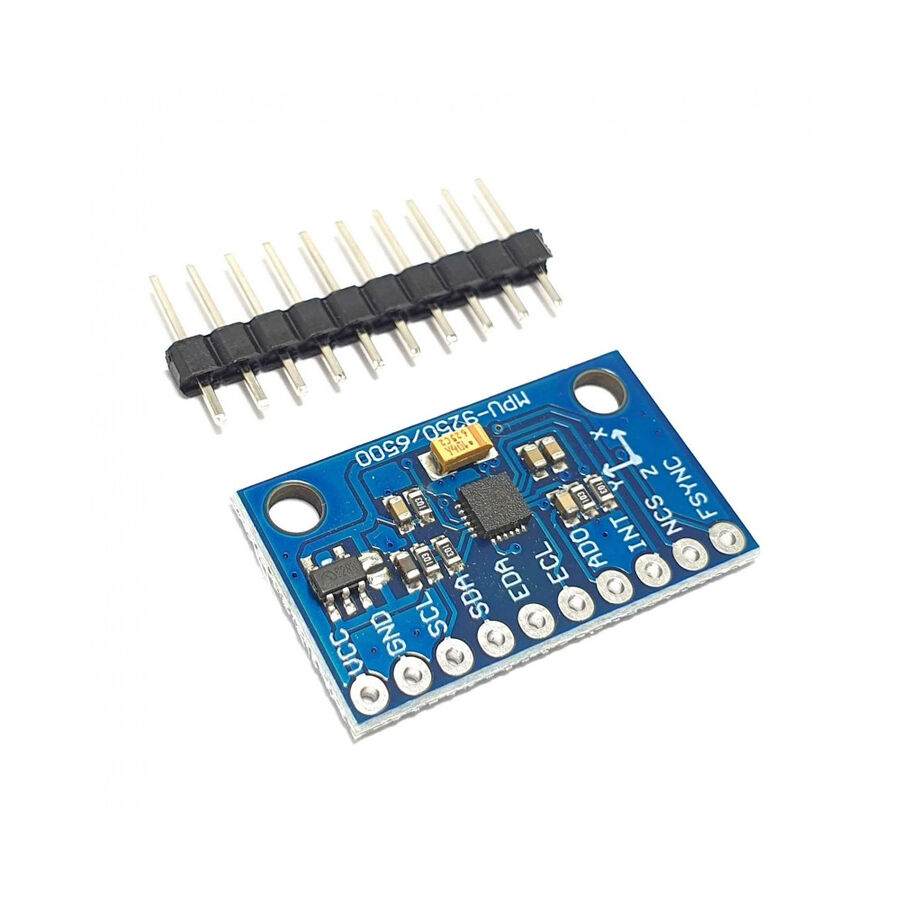
\includegraphics[width=0.5\textwidth]{fig/imu.jpg}
    \caption{ Inertia measurement unit 9 axis}
    \label{IMU} % Unique label for referencing
\end{figure}

\subsection{Barcode Scanner GM65}

\begin{figure}[H]
    \centering
    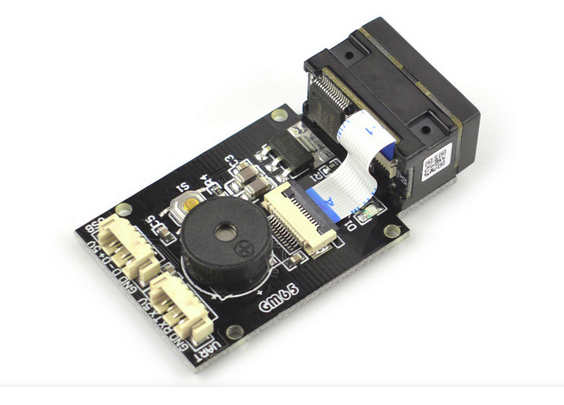
\includegraphics[width=0.5\textwidth]{fig/qr_scanner.png}
    \caption{ Qr code scanner}
    \label{Qr code scanner} % Unique label for referencing
\end{figure}

\subsection{QTRX-HD-11RC}

\begin{figure}[H]
    \centering
    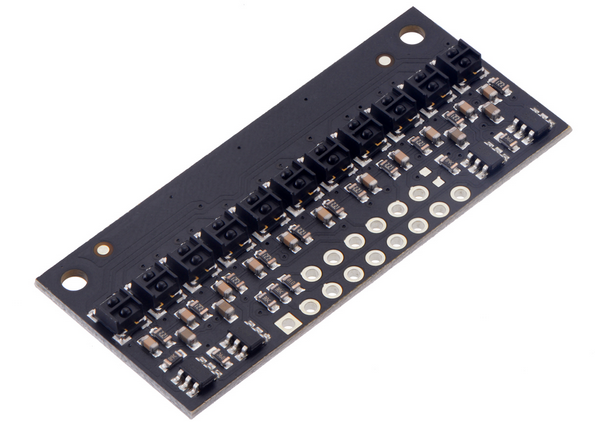
\includegraphics[width=0.5\textwidth]{fig/array.png}
    \caption{ QTRX-HD-11RC Reflectance Sensor Array: 11-Channel }
    \label{QTRX-HD-11RC Ir Array} % Unique label for referencing
\end{figure}


\section{Microcontroller and Communication}

When selecting a microcontroller (MCU), several key factors must be 
considered to ensure it meets the demands of the system. One of the 
most critical criteria is processing power. The system design 
requires an embedded computer capable of running Linux, which is 
essential for implementing the Robot Operating System (ROS). 

ROS provides a robust framework for handling robotic applications, 
including sensor fusion, navigation, and communication between 
various components. Running ROS efficiently requires an embedded 
system with sufficient computational capabilities, including a 
high-performance CPU and adequate RAM.

Another crucial factor is the number of available I/O pins. The 
system involves interfacing with multiple sensors and actuators, 
necessitating a microcontroller with a high pin count to 
accommodate all necessary connections. Many of these devices 
operate using different communication protocols, such as I2C, 
SPI, and UART.

\subsection{Microcontroller and Embedded computer integration}

The AGV's microcontroller and communication system form the backbone 
of its control and data exchange capabilities, ensuring efficient 
processing, seamless communication, and real-time control of the 
robot's operations. 

In this design, the \textbf{Raspberry Pi 4} shown in Figure~\cref{Raspberry Pi 4} serves as the primary 
computational unit, acting as the ``brain'' of the system. Equipped 
with a Linux operating system, it hosts all necessary 
\textbf{ROS (Robot Operating System)} packages, enabling high-level 
decision-making, sensor data processing, and trajectory planning.


\subsubsection{Raspberry Pi 4}

\begin{figure}[H]
    \centering
    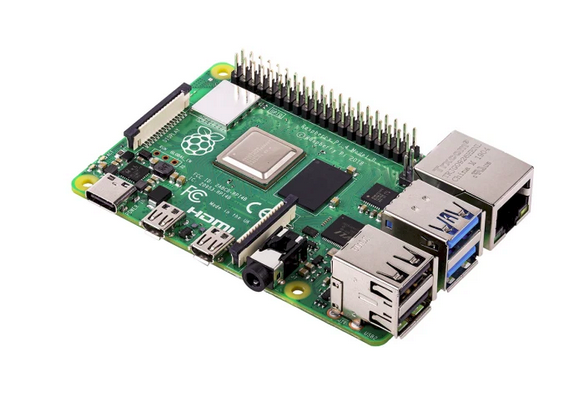
\includegraphics[width=0.5\textwidth]{fig/raspberry.png}
    \caption{ Raspberry Pi 4}
    \label{Raspberry Pi 4} % Unique label for referencing
\end{figure}

Complementing the Raspberry Pi, the \textbf{ESP32 microcontroller} in \cref{ESP32-S3-DevKitC-1} 
supports it by managing low-level tasks 
such as motor control and real-time sensor interfacing. The ESP32 
directly interfaces with motor drivers to regulate speed, 
and direction, ensuring precise actuation of the AGV's propulsion 
system.

Communication between the Raspberry Pi 4 and the ESP32 is achieved 
through a \textbf{serial communication protocol}, which ensures 
reliable and efficient data exchange. This division of responsibilities 
-- high-level computation on the Raspberry Pi and low-level control 
on the ESP32 -- optimizes the system's performance and reliability.

Additionally, the sensors are shared between both components, with 
the ESP32 handling time-sensitive data acquisition and the Raspberry 
Pi performing higher-level processing and integration into the ROS 
framework.

\subsubsection{ESP32-S3-DevKitC-1}

\begin{figure}[H]
    \centering
    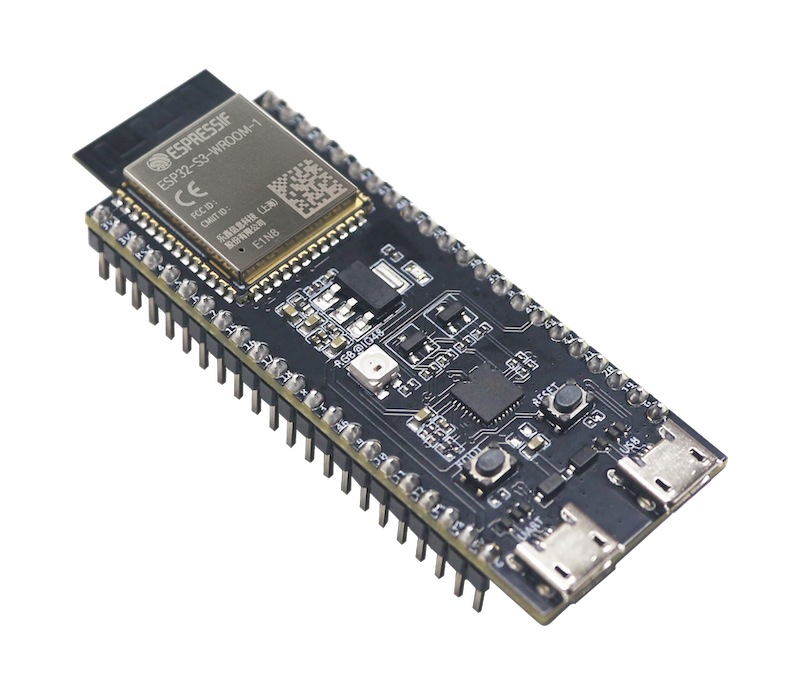
\includegraphics[width=0.5\textwidth]{fig/esp32.png}
    \caption{ ESP32-S3-DevKitC-1}
    \label{ESP32-S3-DevKitC-1} % Unique label for referencing
\end{figure}

\subsubsection{RS232 to Bluetooth Series Adapter}
RS232 to Bluetooth Series Adapter
\begin{figure}[H]
    \centering
    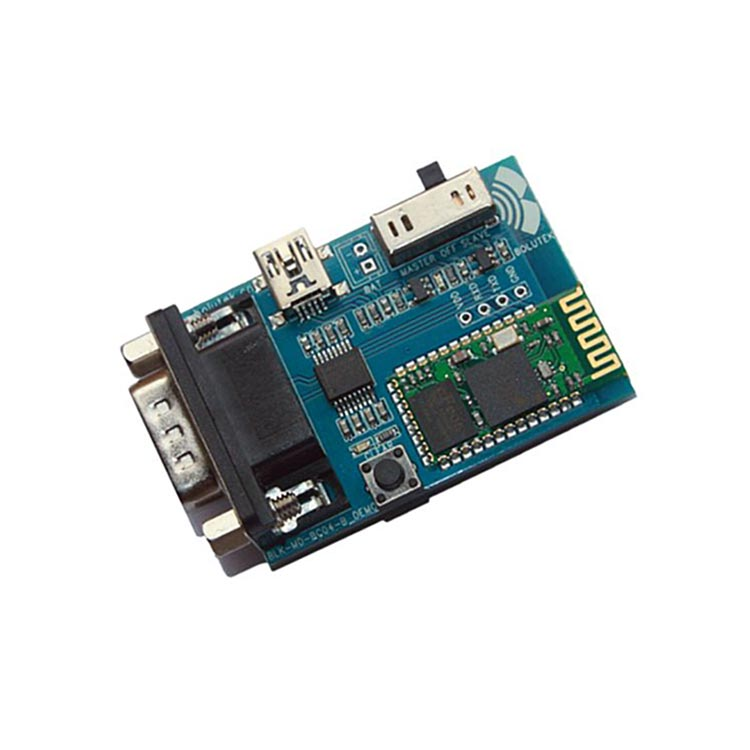
\includegraphics[width=0.5\textwidth]{fig/bluetooth.jpg}
    \caption{ RS232 to Bluetooth Series Adapter}
    \label{RS232 to Bluetooth Series Adapter} % Unique label for referencing
\end{figure}

\subsubsection{TP-Link TL-WR840N}
\begin{itemize}
    \item The \textbf{TP-Link TL-WR840N} is utilized as an access point 
    to facilitate communication between the control unit (PC) and the 
    robot's microcontrollers (Raspberry Pi and ESP32 modules).
    \item By configuring the TL-WR840N as an access point, it creates 
    a wireless network that enables seamless data and command exchange 
    between the PC, Raspberry Pi, and ESP32 modules.
    \item This setup allows for remote control and monitoring of the 
    AGV's operations, enhancing its usability and adaptability.
\end{itemize}

All \textbf{sensors, microcontrollers, and motor drivers} in the AGV 
are selected to work in a \textbf{cohesive and well-integrated system}, 
ensuring seamless communication and efficient operation. 
\textbf{Protocols such as I2C and UART} enable reliable data exchange 
between components, allowing real-time monitoring and control. 
This structured communication enhances \textbf{precision, synchronization, 
and responsiveness}, optimizing the AGV’s navigation, lifting, and 
traction systems while maintaining operational efficiency and safety.
    



% \newpage
% \section{usefull part}
% \begin{figure}[h!]
%     \centering
%     \begin{circuitikz}[scale=1.2, transform shape,american voltages]
  
%         % Wheatstone Bridge
%         \draw (0,0) to [R=$R_1$] (45:3); % Resistor R1
%         \draw (0,0) to [R, l_=$R_2$] (-45:3); % Resistor R3
%         \draw (45:3) to[R=$R_3$] ++(-45:3) coordinate(alpha); % Resistor R2
%         \draw (alpha) to[R=$R_4$] (-45:3); % Resistor R4
  
%         \draw (45:3) --++(0,0.5)  to [short, o-*] ++(-3,0)node[left]{$V_+$}; % Positive terminal
%         \draw (-45:3)--++(0,-0.5)  to [short, o-*] ++(-3,0)node[left]{$V_-$}; % Positive terminal
  
%         % \draw (0,0) to[open, v^=$V_{\text{out}}$, *-*] (alpha);
%         \draw (0,0) to[rmeter, t=$V$] (alpha);
  
  
%     \end{circuitikz}
%     \caption{Load Cell Circuit with Wheatstone Bridge and Amplifier}
%     \label{fig:load-cell}
%   \end{figure}
%   The idea behind the load cell is to use the Wheatstone bridge (\cref{fig:load-cell}). In a Wheatstone bridge, $R_1 = R_2 = R_3 = R_4$, and the output voltage is zero when no force is applied. When weight is applied, it bends the material, which changes the resistivity of the material. This change disrupts the equality of the resistances, causing a difference in voltage across $V$. By experimenting and calibrating with different weights and tracking the changes in voltage, we can measure the weight.

%   It is also worth noting that the signal produced depends on the material properties. If the bending factor is linear, the output will be proportional to the applied weight. However, if the bending becomes exponential (which would be a limitation of the material), the relationship between the applied weight and the output signal may no longer be accurate. Additionally, the placement of the load affects the measurement. The voltage difference across $V$ is used to measure the output of the bridge.
  
%   In theory, we could use the microcontroller's analog input to read the voltage differences. However, the changes are too small to provide an accurate reading. For this reason, the \textbf{HX711} amplifier is used to amplify the signal and convert it into a digital signal.
% \begin{figure}
%     \centering

%     \begin{circuitikz}[american]
%         %
%         \tikzset{myICwl/.style={muxdemux,
%     muxdemux def={Lh=4, Rh=4, w=4,
%     NR=2, NL=2, NB=0, },
%     muxdemux label={L1=IN$(+)$, L2=IN$(-)$,
%     R1=3.3$v$ out, R2=OUT$(-)$,},
%     }
%     }
%     %
%     \tikzset{myICwl2/.style={muxdemux,
%     muxdemux def={Lh=4, Rh=4, w=4,
%     NR=2, NL=2, NB=0, },
%     muxdemux label={L1=IN$(+)$, L2=IN$(-)$,
%     R1=5$v$ out, R2=OUT$(-)$,},
%     }
%     }
%     %
%     \tikzset{myICwl3/.style={muxdemux,
%     muxdemux def={Lh=4, Rh=4, w=4,
%     NR=2, NL=2, NB=0, },
%     muxdemux label={L1=IN$(+)$, L2=IN$(-)$,
%     R1=9$v$ out, R2=OUT$(-)$,},
%     }
%     }
%     %
%     \tikzset{myICwl4/.style={muxdemux,
%     muxdemux def={Lh=4, Rh=4, w=4,
%     NR=2, NL=2, NB=0, },
%     muxdemux label={L1=IN$(+)$, L2=IN$(-)$,
%     R1=24$v$ out, R2=OUT$(-)$,},
%     }
%     }
%     %
%     \tikzset{myICwl5/.style={muxdemux,
%     muxdemux def={Lh=4, Rh=4, w=4,
%     NR=2, NL=2, NB=0, },
%     muxdemux label={L1=IN$(+)$, L2=IN$(-)$,
%     R1=48$v$ out, R2=OUT$(-)$,},
%     }
%     }
%     %
%     \draw (5, 7) node[myICwl5](chip5){MotorobitDC};
%     \draw (5, 4.5) node[myICwl4](chip4){WM-045};
%     \draw (5, 2) node[myICwl3](chip3){LM2596};
%     \draw (5, -0.5) node[myICwl2](chip2){LM2596};
%     \draw (5,-3) node[myICwl](chip1){LM2596};
%     % \draw (5, 2) node[myICwl](chip1){MP1584EN} ;
%     \ctikzset{bipoles/vsourceam/inner plus={ $+$}}
%     \ctikzset{bipoles/vsourceam/inner minus={ $-$}}
%     \draw (chip1.blpin 1)--+(-1,0) coordinate(dist) to[switch,mirror,label=Switch,*-]++(-3,0) to[V, l_=$12V$,-*] ++(0,-2) node[ground]{} coordinate(end);
%     \draw (chip2.blpin 1)--+(-1,0)--(dist);
%     \draw (chip3.blpin 1)--+(-1,0)--(dist);
%     \draw (chip4.blpin 1)--+(-1,0)--(dist);
%     \draw (chip5.blpin 1)--+(-1,0)--(dist);
%     %
%     \draw (chip1.brpin 1)--+(1,0) to[short,l=$3.3V$,-]+(2,0) to [fuse,label=$3A$,-o]+(3,0);
%     \draw (chip2.brpin 1)--+(1,0) to[short,l=$5V$,-]+(2,0)to [fuse,label=$3A$,-o]+(3,0);
%     \draw (chip3.brpin 1)--+(1,0) to[short,l=$9V$,-]+(2,0)to [fuse,label=$1A$,-o]+(3,0);
%     \draw (chip4.brpin 1)--+(1,0) to[short,l=$24V$,-]+(2,0)to [fuse,label=$5A$,-o]+(3,0);
%     \draw (chip5.brpin 1)--+(1,0) to[short,l=$45V$,-]+(2,0)to [fuse,label=$10A$,-o]+(3,0);
%     %
%     \draw (chip1.blpin 2)to node[ground]{}++(-0.5,0);
%     \draw (chip2.blpin 2)to node[ground]{}++(-0.5,0);
%     \draw (chip3.blpin 2)to node[ground]{}++(-0.5,0);
%     \draw (chip4.blpin 2)to node[ground]{}++(-0.5,0);
%     \draw (chip5.blpin 2)to node[ground]{}++(-0.5,0);
    
%     \draw (chip1.brpin 2)to node[ground]{}++(0.5,0);
%     \draw (chip2.brpin 2)to node[ground]{}++(0.5,0);
%     \draw (chip3.brpin 2)to node[ground]{}++(0.5,0);
%     \draw (chip4.brpin 2)to node[ground]{}++(0.5,0);
%     \draw (chip5.brpin 2)to node[ground]{}++(0.5,0);
    
    
%     \end{circuitikz}
%     \caption{Power Distribution Circuit}
% \end{figure}

% \begin{figure}
%     \centering
%     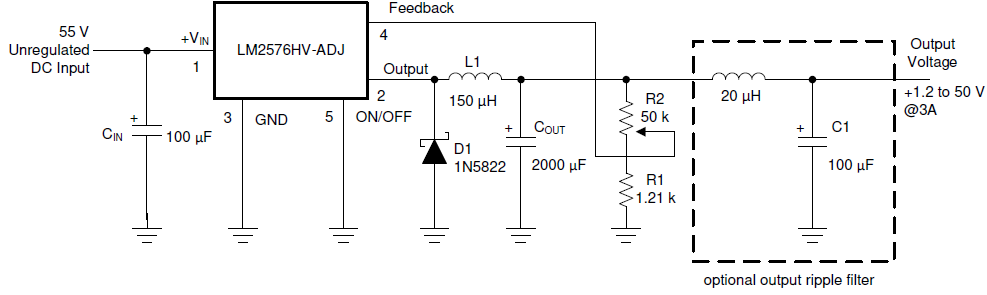
\includegraphics[width=\textwidth]{fig/lm.png}
%     \caption{1.2-V to 55-V Adjustable 3-A Power Supply With Low Output Ripple}
% \end{figure}
% \begin{figure}
%     \centering
%     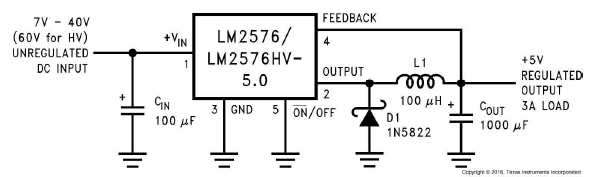
\includegraphics[width=\textwidth]{fig/lm2.png}
%     \caption{Fixed Output Voltage Version Typical Application Diagram}
% \end{figure}

\end{document}